\part{Logique, ensemble et catégorie}
\chapter{Logique}\index{Logique}
La bibliothèque fournit un module pour faire de la logique mathématique indépendamment vue comme extension
des classes fournit par le builtins de Python.
\chapter{Théorie des ensemble}\index{Théorie des ensemble}
\section{Un petit rappel pour les ensembles dans Python}\index{Ensemble dans Python}
La théorie d'ensemble existe sous Python, il suffit simplement de tapez 
\begin{python}
ens = set()
\end{python}
ou écrire simplement 
\begin{python}
 ens = ens = {1, 2, 4}
\end{python}
\section{Théorie des ensembles}\index{Théorie des ensembles}
La notion d'objet immuable en Python est fondamentale,  une structure qui rappel les ensembles en mathématiques que soit fini ou infini est \textit{set}, importante, bien que dans le cadre de SymPy elle s'appui entièrement sur Python avec certain modification, avec la collection d'objet.
\\

\textit{La fonction set accepte donc en argument un objet de type quelconque et s'efforce de le traduire dans un ensemble. Lorsqu'on ne passe aucun argument à set (option 2), ou qu'on lui passe une liste vide, set renvoie naturellement un ensemble vide; on aurait pu utiliser aussi bien, de la même manière, set(()), set({}), ou même set('') pour arriver au même résultat.}

\begin{exercise}
		Définir deux ensembles $X = \lbrace a, b, c, d\rbrace$ et  $Y = \lbrace s, b, d\rbrace$ , puis 			affichez les résultats suivants :
 		\begin{enumerate}
  			 \item les ensembles initiaux.
  			 \item le test d’appartenance de l’élément $c$ à $X$.
  			 \item le test d’appartenance de l’élément $a$ à $Y$.
  			 \item les ensembles $X - Y$ et $Y - X$.
  			 \item l’ensemble $X \cup Y$ (union).
  			 \item l'ensemble $X \cap Y$ (intersection).
	 \end{enumerate}
\end{exercise}

\begin{solution}
Il faut noter qu'il existe une solution qui se base sur le Python builtuints en utilisant la structure de donnée \textit{sets}. Mais comme en n'est dans la logique en utilise 
\begin{python}
from sympy import FiniteSet

X = FiniteSet('a', 'b', 'c', 'd')
Y = FiniteSet('s', 'b', 'd')

class MyClass(Yourclass):
    def __init__(self, my, yours):
        bla = '5 1 2 3 4'
        print bla
\end{python}
\begin{python}
class MyClass(Yourclass):
    def __init__(self, my, yours):
        bla = '5 1 2 3 4'
        print bla
\end{python}

\end{solution}
%%
\subsection{Logique}
\begin{exercise}
Dans la carte de Karnaugh ci-dessous, $X$ indique un terme sans intérêt. Quelle est la forme minimale de la fonction représentée par la carte de Karnaugh?
\end{exercise}
\subsection{Ensembles}
La notion d'objet immuable en Python est fondamentale,  une structure qui rappel les ensembles en mathématiques que soit fini ou infini est \textit{set}, importante, bien que
dans le cadre de SymPy elle s'appui entièrement sur Python avec certain modification, avec la collection d'objet.
\\

\textit{La fonction set accepte donc en argument un objet de type quelconque et s'efforce de le traduire dans un ensemble. Lorsqu'on ne passe aucun argument à set (option 2), ou qu'on lui passe une liste vide, set renvoie naturellement un ensemble vide; on aurait pu utiliser aussi bien, de la même manière, set(()), set({}), ou même set('') pour arriver au même résultat.}

	\begin{exercise}
		Définir deux ensembles $X = \lbrace a, b, c, d\rbrace$ et  $Y = \lbrace s, b, d\rbrace$ , puis 			affichez les résultats suivants :
 		\begin{enumerate}
  			 \item les ensembles initiaux.
  			 \item le test d’appartenance de l’élément $c$ à $X$.
  			 \item le test d’appartenance de l’élément $a$ à $Y$.
  			 \item les ensembles $X - Y$ et $Y - X$.
  			 \item l’ensemble $X \cup Y$ (union).
  			 \item l'ensemble $X \cap Y$ (intersection).
	 \end{enumerate}
	\end{exercise}

\begin{solution}
Il faut noter qu'il existe une solution qui se base sur le Python builtuints en utilisant la structure de donnée \textit{sets}. Mais comme en n'est dans la logique en utilise 
\begin{python}
from sympy import FiniteSet

X = FiniteSet('a', 'b', 'c', 'd')
Y = FiniteSet('s', 'b', 'd')

class MyClass(Yourclass):
    def __init__(self, my, yours):
        bla = '5 1 2 3 4'
        print bla
\end{python}
\begin{python}
class MyClass(Yourclass):
    def __init__(self, my, yours):
        bla = '5 1 2 3 4'
        print bla
\end{python}

\end{solution}
%\begin{exercise}
%Si $P$, $Q$, $R$ sont des sous-ensembles de l'ensemble universel $U$, alors $(P \cap Q\capR) \cup (P^{c} \cap Q \cap R)\cup(Q^{x}\cupR^{x})$ si
%\begin{enumerate}
%  \item  
%  \item 
%  \item
%\end{enumerate}
%\end{exercise}
%-----------------------------------------------
\chapter{Théorie des catégories}
\section{Note historique}
Les catégories sont utilisées dans la plupart des branches mathématiques et dans certains secteurs de l'informatique théorique et en mathématiques de la physique. Elles forment une notion unificatrice. Cette théorie a été mise en place par Samuel Eilenberg et Saunders Mac Lane en 1942-1945, en lien avec la topologie algébrique, et propagée dans les années 1960-1970 en France par Alexandre Grothendieck, qui en fit une étude systématique. À la suite des travaux de William Lawvere, la théorie des catégories est utilisée depuis 1969 pour définir la logique et la théorie des ensembles ; la théorie des catégories peut donc, comme la théorie des ensembles ou la théorie des types, avec laquelle elle a des similarités, être considérée comme fondement des mathématiques. Une élaboration fine est développé avec l'ajout de la théorie d'homotopie pour en donnée de la théorie des types homotopiques qui sera pas traité dans ce chapitre  ni d'une catégorie élaboré tel-que: 2-catégorie ou $\infty$-catégorie
\section{Introduction}
Dans le langage des catégories tout commence avec la relation des objets entre-eux à travers des flèches ou morphismes.
\\

Application à l'informatique.
\\

Pour commencer nous définissions des objets et des flèches qui met en relation avec ces objets 

\begin{example}(Produit cartésien)
Comment définir le produit cartésien $A \times B = \left\lbrace \left( a, b\right)  \vert a \in A \wedge b \in B\right\rbrace$ sans faire intervenir $\in$, en considérant uniquement des transformations(fonctions) entre objects(ensembles)?.
\begin{itemize}
 \item premier projection: $\pi_{1}: A \times B \rightarrow A$
 \item deuxième projection: $\pi_{2}: A \times B \rightarrow B$
 \item la structure $\left(A \times B,\pi_{1},\pi_{2}\right) $ est optimale
 \item quelques soient $f: C \rightarrow A$ et $g: C \rightarrow B$ on peut construire 
 $\langle f, g \rangle: C \rightarrow A \times B$ définie par et $\langle f, g \rangle\left(x\right)=\left(f\left(x\right),g\left(x\right)\right)$
 \\
 
 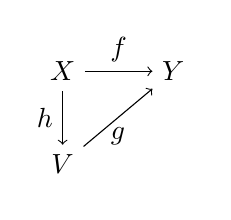
\begin{tikzpicture}[every node/.style={midway}]
\matrix[column sep={4em,between origins},
    row sep={2em}] at (0,0)
{ \node(X)   {$X$}  ; & \node(Y) {$Y$}; \\
\node(V) {$V$};                   \\};
\draw[<-] (V) -- (X) node[anchor=east]  {$h$};
\draw[->] (V) -- (Y) node[anchor=north]  {$g$};
\draw[->] (X)   -- (Y) node[anchor=south] {$f$};
\end{tikzpicture}
\end{itemize}
Le code python correspondant.
\begin{python}
from sympy.categories import Object, NamedMorphism
from sympy import init_printing(pretty_print=True)
A = Object("A")
B = Object("B")
\end{python}
\end{example}
